\section{Integrated assessment against CN4252}\label{sec:cn4252-assessment}

\subsection{Integrated carbon result}
\begin{table}[htbp]\centering\small
\caption{Plain-language carbon comparison on the verified common-output screening boundary. The avoided total reflects the combined candidate architecture---nuclear heat substitution, carbon capture and lower natural-gas use---with lifecycle burdens included; it is not attributed to nuclear heat alone.}
\begin{tabular}{p{0.46\linewidth}p{0.38\linewidth}}
\toprule Quantity & Verified value \\ \midrule
Baseline natural gas & 52.5 MMSCFD~\cite{inltev953}\\
Candidate natural gas & 34.0 MMSCFD~\cite{inltev961}\\
Natural-gas reduction & 18.5 MMSCFD\\
Baseline direct CO$_2$ & approximately 902,060 t/y\\
Candidate direct CO$_2$ & approximately 39,966 t/y\\
Direct CO$_2$ avoided & approximately 862,094 t/y\\
Lifecycle CO$_2$e avoided & approximately 917,139 tCO$_2$e/y\\
Candidate lifecycle intensity & approximately 1.95 kgCO$_2$e/kgH$_2$\\
Annual hydrogen output & approximately 97,946 t/y\\
\bottomrule
\end{tabular}
\end{table}

\subsection{Integrated cost result}
\begin{table}[htbp]\centering\small
\caption{Cost changes represented by the canonical screening model. Negative means an avoided expenditure; positive means an added represented burden.}
\begin{tabular}{p{0.57\linewidth}r}
\toprule Annual term & Change (S\$ million/y) \\ \midrule
Natural-gas expenditure avoided & $-94.831$\\
Reactor/source economic burden added & $+76.572$\\
CCS annualisation added & $+10.683$\\
Integration/site allowance added & $+2.857$\\
CO$_2$ transport and storage added & $+8.135$\\
Project electricity revenue & $0.000$\\ \midrule
Net represented incremental annual cost & $+3.416$\\
\bottomrule
\end{tabular}
\end{table}

The resulting approximately S\$3.725/tCO$_2$e is a \textbf{screening abatement cost}, not a turnkey Singapore nuclear-project quotation or bankable First-of-a-Kind (FOAK) estimate. Important unresolved project costs include Singapore construction/site premium, financing, Engineering, Procurement and Construction (EPC), licensing, security, detailed IHX qualification, emergency planning, insurance/liability, waste/decommissioning, schedule risk, contingency and contracted CCS infrastructure.


\subsection{Assessment against the official CN4252 requirements}
The official problem statement requires a solution at scale to reduce more than 0.25 MtCO$_2$e/y within Singapore at less than S\$100/tCO$_2$e, clearly explain the abatement mechanism and implementation roadmap, and is assessed on feasibility, potential effectiveness, accuracy and presentation.

\begin{table}[htbp]\centering\small
\caption{Direct mapping to the official CN4252 problem statement.}
\begin{tabular}{p{0.28\linewidth}p{0.25\linewidth}p{0.37\linewidth}}
\toprule Official requirement & Project result & Status / interpretation \\ \midrule
Abatement $>0.25$ MtCO$_2$e/y & $\sim0.917$ MtCO$_2$e/y & Numerical screening threshold exceeded\\
Cost $<\mathrm{S\$}100$/tCO$_2$e & $\sim\mathrm{S\$}3.725$/tCO$_2$e & Screening threshold satisfied\\
How emissions are abated & Nuclear heat substitution + CCS + reduced natural-gas demand; lifecycle burdens included & Explicit carbon ledger\\
Implementation roadmap & Staged decision gates in Section 10 & Explicit roadmap\\
Feasibility & Conditional across engineering, safety, regulation, siting and CCS & Not a deployment approval\\
Potential effectiveness & $\sim0.917$ MtCO$_2$e/y plus bounded sensitivities & Supported within model\\
Accuracy & Primary sources + assumptions + equations + Rust + provenance + CI + independent reviews & Traceable/reproducible\\
Presentation & Three orientation figures + ledgers + requirement mapping & Submission-facing explanation\\
\bottomrule
\end{tabular}
\end{table}

\noindent\textbf{CONDITIONAL MODEL PASS.} The numerical screening requirements are satisfied under the declared model boundary. This does not demonstrate commercial Singapore deployment, nuclear licensing approval, a selected Jurong site, a Singapore Emergency Planning Zone, project Probabilistic Risk Assessment/mechanistic source term, a qualified commercial 176.8 MWth IHX, site-specific nuclear/chemical Quantitative Risk Assessment, guaranteed cross-border CCS, or bankable FOAK economics.


\subsection{Result interpretation}
The verified final-design calculation produces approximately 97,946 tH$_2$/y at 85\% availability. Direct avoided emissions are approximately 862,094 tCO$_2$/y. Lifecycle avoided emissions are larger, approximately 917,139 tCO$_2$e/y, because the candidate consumes less natural gas than the same-output conventional baseline and therefore also avoids upstream gas-supply emissions. Captured CO$_2$ is not added again to the avoided-emissions numerator.

\begin{table}[htbp]\centering\small
\caption{Principal submission-facing final-design result. Electricity export receives zero value because no validated project off-design power output is claimed.}
\label{tab:final-result}
\begin{tabular}{p{0.39\linewidth}p{0.27\linewidth}p{0.25\linewidth}}
\toprule
Quantity & Verified screening result & Basis \\
\midrule
Reformer / supplied heat & 871$^\circ$C / 900$^\circ$C & INL~\cite{inltev953,inltev961} \\
Hydrogen production & 97,946 t/y & Eq.~\ref{eq:annual-h2} \\
INL process heat & 176.8 MWth & INL~\cite{inltev961} \\
Selected reactor architecture & 600 MWth GTHTR300C class & Nishihara~\cite{nishihara2007potential} \\
Nishihara source heat branch & 370 MWth & Nishihara~\cite{nishihara2007potential} \\
Remaining reactor thermal capacity & 423.2 MWth; no power claim & Eq.~\ref{eq:remaining-thermal} \\
CO$_2$ captured & 542,362 t/y & Eq.~\ref{eq:captured-annual} \\
Direct CO$_2$ avoided & 862,094 t/y & Eq.~\ref{eq:direct-avoided} \\
Lifecycle CO$_2$e avoided & 917,139 t/y & Eq.~\ref{eq:lifecycle-reconciliation} \\
Candidate lifecycle intensity & 1.95 kgCO$_2$e/kgH$_2$ & Eq.~\ref{eq:lifecycle-intensity} \\
Project electricity revenue & S\$0/MWh & Assumption A-17 \\
Annual incremental cost & approximately S\$3.416 million/y & Eq.~\ref{eq:annual-incremental-cost} \\
Abatement cost & approximately S\$3.725/tCO$_2$e & Eq.~\ref{eq:abatement-cost-final} \\
CN4252 abatement criterion & $>250,000$ tCO$_2$e/y: PASS & assignment requirement \\
CN4252 cost criterion & $<\mathrm{S\$}100$/tCO$_2$e: PASS & assignment requirement \\
Joint classification & \textbf{CONDITIONAL MODEL PASS} & derived interpretation \\
\bottomrule
\end{tabular}
\end{table}

\noindent\textit{Numerical basis for Table~\ref{tab:final-result}.} The 871/900$^\circ$C temperatures, 176.8 MWth duty, 130-MMSCFD service and source CO$_2$/natural-gas rates are INL source values~\cite{inltev953,inltev961}. The 600-MWth reactor and approximately 370-MWth heat branch are GTHTR300C design-study values~\cite{nishihara2007potential}. The 423.2 MWth value is the project subtraction $600-176.8$, not an external measurement. Hydrogen tonnes per year, captured/direct/lifecycle CO$_2$, lifecycle intensity, annual incremental cost and abatement cost are project-derived Rust outputs whose input-by-input substitutions are given in Section~\ref{sec:ledgers} and the master provenance register. S\$0/MWh is the conservative project boundary adopted because no validated off-design export model exists.


\subsection{Why lifecycle avoidance exceeds direct avoidance}
The annual-abatement threshold is exceeded by approximately 667,139 tCO$_2$e/y. Equivalently, 0.917 MtCO$_2$e/y is about \textbf{3.7 times} the required 0.25 MtCO$_2$e/y. Lifecycle avoidance exceeds direct avoidance by about 55 ktCO$_2$e/y: the reduction in upstream natural-gas burden is larger than the added nuclear-heat, auxiliary-electricity and CO$_2$ transport/storage lifecycle burdens.

\begin{figure}[htbp]\centering
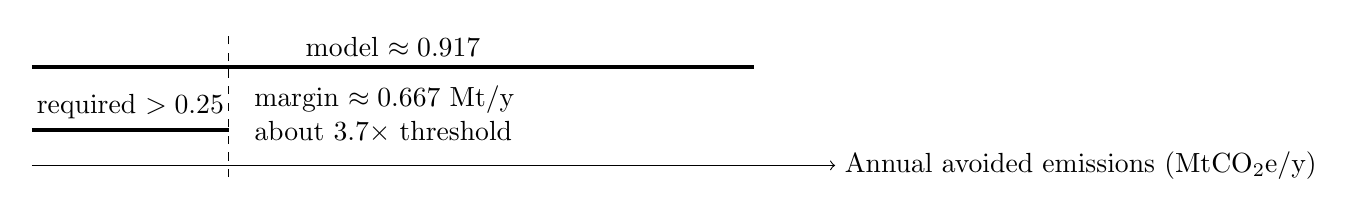
\begin{tikzpicture}[x=1cm,y=1cm]
\draw[->] (0,0)--(10.2,0) node[right]{Annual avoided emissions (MtCO$_2$e/y)};
\draw[very thick] (0,0.45)--(2.5,0.45) node[midway,above]{required $>0.25$};
\draw[very thick] (0,1.25)--(9.17,1.25) node[midway,above]{model $\approx0.917$};
\draw[dashed] (2.5,-0.15)--(2.5,1.65);
\node[align=left,anchor=west] at (2.7,0.65) {margin $\approx0.667$ Mt/y\\about 3.7$\times$ threshold};
\end{tikzpicture}
\caption{CN4252 annual-abatement test using the independently verified final lifecycle result. The model result is a conditional screening result, not measured project performance.}
\label{fig:abatement-threshold}
\end{figure}


\subsection{Economic robustness}
Abatement cost asks how much additional annual cost is associated with each tonne of lifecycle emissions avoided. Its definition is given by Eq.~\ref{eq:abatement-cost-definition}, and the full numerical substitution is Eq.~\ref{eq:abatement-cost-final}.
The controlling case gives no monetary credit to uncertain project electricity output but still charges the full selected reactor source-product economic burden. Its approximately S\$3.725/tCO$_2$e result is about S\$96.3/t below the S\$100/t ceiling. Thus the numerical cost pass does not depend on electricity revenue.

\begin{figure}[htbp]\centering
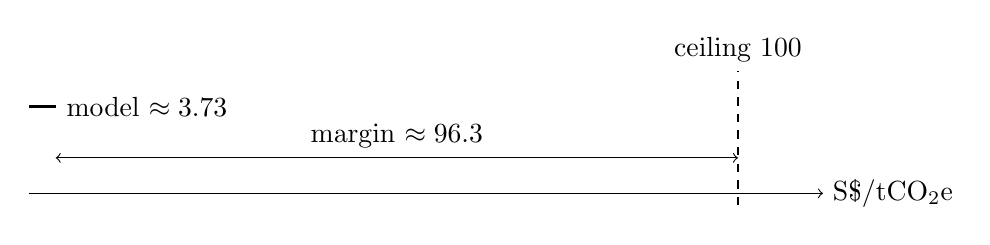
\begin{tikzpicture}[x=0.09cm,y=1cm]
\draw[->] (0,0)--(112,0) node[right]{S\$/tCO$_2$e};
\draw[very thick] (0,1.1)--(3.725,1.1) node[right]{model $\approx3.73$};
\draw[dashed] (100,-0.15)--(100,1.55) node[above]{ceiling 100};
\draw[<->] (3.725,0.45)--(100,0.45) node[midway,above]{margin $\approx96.3$};
\end{tikzpicture}
\caption{CN4252 abatement-cost test for the controlling zero-electricity-revenue case.}
\label{fig:cost-threshold}
\end{figure}


\subsection{Conditional model pass}
The final configuration satisfies both numerical assignment thresholds under the declared source/design-study and lifecycle assumptions. It remains a \textbf{CONDITIONAL MODEL RESULT}, not evidence of an existing Singapore commercial project.

